\chapter{Module 6 \hspace{0.5em} Electromagnetism}

\section{Introduction to Electromagnetism} \label{07/02/25}
	\def\arraystretch{1.5}
	\begin{table}[htbp]
		\centering
		\begin{tabular}{p{0.15\linewidth}|p{0.24\linewidth}|p{0.24\linewidth}|p{0.24\linewidth}}
			\hline
			 & Gravitational Field & Electric Field & Magnetic Field \\ \hline
			Surrounds... & mass & charge & magnet or electric current \\
			Exerts force on & other masses & other charges & other magnets, magnetic materials, or moving electric charges \\
			Direction of a field is determined by... & the direction of the force on a test mass in the field & the direction of the force on a positive test charge in the field & the direction of the force on a test north pole in the field \\
			Field vector & $g$, units: \si{\newton\per\kilogram}, \si{\metre\per\second\squared} & $E$, units: \si{\newton\per\coulomb} or \si{\volt\per\meter} & $B$, units:\si{\newton\metre\per\ampere} or \si{\tesla} \\
			Uniform field exists... & inside a room on the Earth's surface ie. a small enclosed system on a large mass & between two parallel charged plates & between the poles of a large horseshoe magnet, or inside a coil carrying an electric current \\ \hline
		\end{tabular}
	\end{table}

	\subsection{Charged Particles in Uniform Electric Fields}
		\begin{itemize}
			\item A uniform electric field occurs between two parallel plates of opposite and equal charges
			\item The potential difference between the plates, $\Delta V$, is measured as the change in potential over the field, not the value of the potential at a given point.
			\item It is the \textbf{change in potential energy} as a result of \textbf{work} being done on the charge
		\end{itemize}

		$$V_f - V_i = Fd = -Ed$$

		Moving a positive charge \textbf{against} the field requires work ($W=Fs$). When a charge is moved in an electric field it experiences a change in potential. The potential difference is defined as \textbf{the work done per unit charge}

	\subsection{Acceleration of Charged Particles due to an Electric Field}
		\begin{itemize}
			\item Electric field is an electrostatic force, $E=Fq$
			\item The acceleration experienced by a charge is given by $F=ma$
		\end{itemize}
		\begin{align*}
			F &= ma \\
			E &= \frac{F}{q} \\
			F &= Eq \\
			ma &= Eq \\
			a &= \frac{Eq}{m}
		\end{align*}

	\subsection{Work Done on a Charge}
		Work is done \textbf{by} the field \textbf{on the particle} when the charge moves through a potential difference $\Delta V$
		\begin{align*}
			W &= Fd \\
			F &= qE \\
			W &= qEd
		\end{align*}
		\begin{align*}
			\because E &= -\frac{\Delta V}{d} \\
			-\Delta V &= Ed \\
			W &= qEd = -1 \Delta V
		\end{align*}

	\subsection{Acceleration on a Charge}
		In a uniform field, F is constant, $\therefore a = \text{constant}$
		\begin{align*}
			u_{\perp} &= u\sin{\theta} \\
			u_{\parallel} &= u\cos{\theta} \\
			v_{\parallel} &= u_{\parallel} + \frac{Eq}{m}t \\
			v_\perp &= u_\perp + a_\perp t \\
			v_\perp &= u_\perp
		\end{align*}

\section{Charged Particles in a Uniform Magnetic Field} \label{10/02/2025}
	Conventional current = direction of a positive charge
	$$F = qvB \sin{\theta}$$
	where, $B = \text{magnetic field strength}$, $v = \text{velocity of the charge}$, and $q = \text{charge}$

\section{Practical Investigation 6.1 - A current-carrying conductor in a uniform magnetic field, force versus current} \label{20/02/2025}
	\textbf{Aim:} To investigate the relationship between force and current for a current carrying conductor in a magnetic field.

	\subsection{Materials}
		\begin{itemize}
			\item Current balance
			\item Connecting wires
			\item Ammeter
			\item Rheostat
			\item Power supply
			\item Ruler
		\end{itemize}
	
	\subsection{Variables}
	
		\begin{table}[htbp]
			\centering
			\begin{tabular}{l|l}
				Independent	& Current \\
				Dependent	& Mass required to balance \\
				Control		& Temperature, voltage, length inside solenoid, magnetic field strength
			\end{tabular}
		\end{table}
	
	\subsection{Risk Assessment}
	
		\begin{table}[htbp]
			\centering
			\begin{tabular}{l|l}
				Hazard			& Precaution \\ \hline
				Electrocution		& Turn off power supply while modifying circuit \\
				Damage to equipment	& Keep devices away from solenoid
			\end{tabular}
		\end{table}

	\subsection{Method}
		\begin{enumerate}
			\item Set up the current balance
			\item With no current flowing, level the current balance
			\item Position the solenoid around the current balance
			\item Connect a power supply and ammeter to the current balance. A second power supply should be connected to the solenoid.
			\item Increase the current into the balance and re-level it using masses.
			\item Record the mass required to level the balance depending on the current flow
		\end{enumerate}
	
	\subsection{Results}
		\begin{table}[htbp]
			\centering
			\begin{tabular}{l|l|l}
				Current	& Mass	& Force \\ \hline
				0.5 	& 0.060	& 0.00059	\\
				1	& 0.072	& 0.00071	\\
				1.5	& 0.084	& 0.00082	\\
				2	& 0.096	& 0.00094	\\
				2.5	& 0.11	& 0.0011	\\
				3	& 0.12	& 0.0012	\\
				3.5	& 0.12	& 0.0012
			\end{tabular}
		\end{table}

		\begin{align*}
			B &= \frac{\mu_0 N I}{L} \\
			  &= \frac{\mu_0 \times 700 \times I}{0.15}
		\end{align*}
		\begin{align*}
			F &= BIl \sin{\theta} \\
			\frac{F}{I} &= Bl = \text{gradient} \\
				    &= B \times 0.025
		\end{align*}

	\subsection{Data and Analysis}
		\begin{enumerate}
			\item \textbf{When investigating the relationship between force and current, what angle should the wire along the end of the current balance make with the magnetic field? Why?}

				The wire at the end of the current balance should be perpendicular to the magnetic field so that the maximum force is generated, ie. $\sin{\theta}=1$

			\item \textbf{Why can the effect of the connection wires along the length of the current balance be ignored?}
				
				The connection along the length of the current is parallel to the magnetic field and therefore experiences no force. Therefore, it does not affect the result.

			\item \textbf{Calculate the force corresponding to each measurement of mass and record it in the corresponding column of the results. How is force calculated?}
				
				$$F_B = mg$$

			\item \textbf{Determine the equation of the relationship between the force and current of the data}

				Force is directly proportional to current. From the graph, $F = 2.48 \times 10^{-4} I$
		
		\end{enumerate}
	
	\subsection{Conclusion}
		\begin{enumerate}
			\item \textbf{What is the nature of the relationship between these two variables?}

				Force and current have a linear relationship.

			\item \textbf{What does this say about how changes in the current will affect the force acting on a wire that is in a magnetic field?}

				Force is directly proportional to current.

			\item \textbf{What is the significance of the gradient of the graph? How reliable was the value you found}

				The gradient of the graph shows the relationship between force and current. The data was very reliable.

		\end{enumerate}

\section{Practical Investigation 6.2 - Parallel wires, quantitative data analysis} \label{24/02/2025}

	\textbf{Aim:} To quantitatively analyse the way two parallel current-carrying conductors interact.

	\subsection{Data and Analysis}
	
		\begin{enumerate}
			\item \textbf{What will be the ratio of the current in the top wire to that in the bottom wire?}
				The ratio is one to one.

			\item \textbf{Will the wires attract or repel? Explain your answer.}
				Consider the bottom rod. By right hand grip rule, the magnetic field above the rod is into the page. Due to the motor effect, the top wire experiences an upwards force. Similarly, the top wire has a magnetic field into the page that exerts a downward force on the bottom wire. Therefore, the two wires are repelled from each other.

			\item \textbf{The cables are now brought toward each other and the force per unit length between them is measured. Assuming that the power supply is supplying a constant 10A of current, complete the following table for the variation in distance.}

				\begin{table}[htbp]
					\centering
					\begin{tabular}{l|l}
							Distance $d$ (cm)	& $\frac{F_B}{l}$ (Nm$^{-1}$) \\ \hline
							30			& $6.67 \times 10^{-7}$ \\
							25			& $8.00 \times 10^{-7}$ \\
							20			& $1.00 \times 10^{-6}$ \\
							15			& $1.33 \times 10^{-6}$ \\
							10			& $2.00 \times 10^{-6}$ \\
							5			& $4.00 \times 10^{-6}$ \\
							1			& $2.00 \times 10^{-5}$
					\end{tabular}
				\end{table}

			\begin{figure}
				\centering
				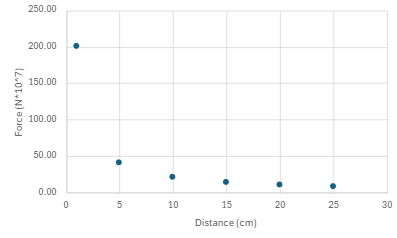
\includegraphics[width=15cm]{prac 6.2.png}
				\caption{Force over Distance graph}
			\end{figure}

			\item \textbf{At what distance apart would the force due to the magnetic field around each wire be sufficient to balance the mass of the top wire? Assume that the wires are straight and the lower wire is unable to move away.}
			
				\begin{align*}
					m &= 1540 \times 0.001 \\
					  &= 1.54 \text{kg}
				\end{align*}

				\begin{align*}
					F_G &= ma \\
					    &= 1.54 \times 9.8 \\
					    &= 15.1 \text{N}
				\end{align*}
				
				\begin{align*}
					F_B &= \frac{\mu_0 I}{2 \pi r} \times l \times I \\
					    &= \frac{\mu_0 I^2 l}{2 \pi r} \\
					r &= \frac{\mu_0 I^2 l}{2 \pi F_B}
				\end{align*}

				\begin{center}
					Let $F_B = F_G$
				\end{center}
				
				\begin{align*}
					r &= \frac{\mu_0 I^2 l}{2 \pi F_G} \\
					  &= 0.133 \times 10^{-6} \text{ m}
				\end{align*}

			\item \textbf{The cable is designed to support a maximum continuous current of 110A. If the cable were carrying this current, at what distance would the force between the wires balance the mass of the top wire?}

				\begin{align*}
					r &= \frac{\mu_0 I^2 l}{2 \pi F_G} \\
					  &= 1.60 \times 10^{-4}
				\end{align*}

			\item \textbf{If the force experienced by the top wire is exactly balancing the force due to gravity, would the force experienced by the bottom wire be larger, the same, or small? Explain your answer.}

				The net force of the bottom wire would be greater. The top wire is not fixed in place and still has no acceleration, therefore has a net force of 0. The bottom wire experiences a repulsion force and the force of gravity in the same direction, therefore has a greater net force.
		\end{enumerate}


\section{Electromagnetic Induction} \label{04/03/2025}

	\subsection{Faraday's Law}
		\begin{figure}[htbp]
			\centering
			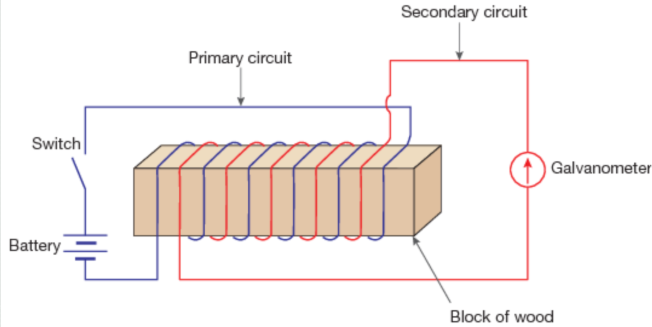
\includegraphics[width=15cm]{faradays_law.png}
		\end{figure}

		\begin{itemize}
			\item When the primary circuit is closed, a small current is momentarily registered in the secondary circuit
			\item When the current in the primary coil was turned off, the same observation was made in the secondary coil but in the opposite direction
			\item When the current in the primary circuit was consistent, no current was detected in the secondary coil
			\item Both circuits produce a magnetic field with opposite polarities
		\end{itemize}
		
		Faraday's law states that:

		\begin{center}
			\Large The induced emf in a circuit is equal in magnitude to the rate at which the magnetic flux through the circuit is changing with time
		\end{center}

		\begin{align*}
			\epsilon = -n \frac{\Delta \phi}{\Delta t}
		\end{align*}

\newpage

\section{Information Retrieval} \label{10/03/2025}

	\begin{enumerate}
		\item \textbf{What is magnetic flux?}

			Flux is the amount of field lines passing through a surface

		\item \textbf{What is required for electromagnetic induction?}
		
			\begin{itemize}
				\item Change in flux
				\item Conductor
				\item Magnet
				\item Relative motion between magnet and conductor
			\end{itemize}

		\item \textbf{How is relative motion between magnetic field and conductor achieved?}
		
			\begin{itemize}
				\item Physically move magnet and coil away from each other
				\item Change current in the primary coil
				\item Change the magnetic field strength (magnetic flux density)
				\item Change the magnetic field direction
			\end{itemize}

		\item \textbf{How can a change in magnetic flux be created?}
		
			Same as above

		\item \textbf{State Lenz's Law}
		
			Magnetic field produced by the induced current opposes change in flux.

		\item \textbf{Describe the steps to determine the direction of an induced current.}
		
			\begin{enumerate}
				\item Find the change in flux
				\item Determine the direction of the magnetic field that needs to be produced to oppose the change in flux
				\item Determine the direction of the induced emf/current using right hand palm rule
				\item Describe the effect
			\end{enumerate}

		\item \textbf{State the motor effect}
		
			A current carrying conductor in an external magnetic field experiences a force
	\end{enumerate}

\section{Back EMF}

	From electromagnetic induction:
	\begin{itemize}
		\item A conductor experiencing a changing magnetic flux will produce an emf
		\item In a motor the supply voltage causes the coil to experience motor effect, resulting in torque
		\item As the coil rotates there is relative motion between the conductor and the magnetic field, ie. the coil experiences a change in magnetic flux
		\item By Faraday's Law, the changing magnetic flux induces an emf in the coil
		\item By Lenz's Law, the current produced by this induced emf will produce a magnetic field that opposes the change in magnetic flux
		\item \textbf{Hence}, the induced current will be in the opposite direction to the supply current
		\item The emf that a motor generates opposes the supply emf is called the \textbf{back emf}
	\end{itemize}

	\begin{align*}
		\epsilon_{in coil} = \epsilon_{supplied} - \epsilon_{back}
	\end{align*}

	Effect of back emf:
	\begin{itemize}
		\item The rate of change of flux experienced by the coil increases with the speed of rotation
		\item $\therefore$ back emf also increases with speed of rotation
		\item This back emf reduces the net emf across the coil
		\item Hence, the current is reduced
		\item Torque due to supply current is reduced
		\item Torque from induced current (due to back emf) increases until the torques are balanced, $F_{net} = 0$
	\end{itemize}

	When the motor is first switched on, before the rotation starts:
	\begin{itemize}
		\item There is no back emf (no relative motion between coil and magnetic field)
		\item There is a large current flowing through the coil
		\item Large current produces large torque, spins fast
		\item As motor spins faster, back emf increases until it is equal to supply emf
		\item When this occurs, there is no voltage across the coil and therefore no current flowing through the coil
		\item No current, therefore no net force, therefore constant rate (Newton's first law)
	\end{itemize}

\section{Example HSC Question} \label{11/03/2025}

	\textbf{Question 21 (3 marks)}

	A fan that ventilates an underground mine is run by a very large DC motor. This motor is connected in series with a variable resistor to protect the windings in the coil.

	When the motor is starting up, the variable resistor is adjusted to have a large resistance. The resistance is then lowered slowly as the motor increases to its operating speed.

	Explain why no resistance is required when the motor is running at high speed, but a substantial resistance is needed when the motor is starting up.



	\textbf{Answer:} A variable resistor is required when the motor is starting up because the supplied current will be high and high resistance limits the current. This prevents motor burnout.

	When the motor is at operational speed, the coil is rotating relative to a magnetic field and induced emf (back emf) is produced, reducing the current.

\newpage

\section{Effects of Back EMF - motor burn out}

	When a heavier mechanical load is placed on the motor,

	\begin{itemize}
		\item Rotational speed decreases
		\item Back emf decreases
		\item Current increases
		\item Torque and rotational speed increase until new equilibrium is reached
	\end{itemize}

	When armature is prevented from moving,
	\begin{itemize}
		\item No back emf due to no $\frac{\Delta \phi}{\Delta t}$
		\item Large current
		\item Resistance $\rightarrow$ heat $\rightarrow$ motor burn out
	\end{itemize}

\section{Eddy Currents} \label{12/03/2025}

	Induced currents do not occur only in coils and wires. They can also occur:

	\begin{itemize}
		\item when there is a magnetic field acting on part of a metal object and there is relative motion between them
	\end{itemize}

\section{Transformers}

	\begin{itemize}
		\item Devices that increase or decrease AC voltage by mutual induction
		\item Consists of two coils of insulated wire called the \textbf{primary and secondary coils}
		\item The size on the emf depends on the number of turns in the secondary coil: $\varepsilon = -n \frac{\Delta \phi}{\Delta t}$l
		\item An AC voltage is placed on the primary coil
		\item If there are less turns in the secondary coil, there is less current
	\end{itemize}

	\subsection{Ideal Transformers}
	
		If the transformer is ideal, it is 100\% efficient and the energy input at the primary coil is equal to the energy output of the secondary coil.
		
		To prevent eddy currents, the iron core must be split and laminated to form donuts (parallel to the direction of the coils)(idk how to word this)

		\subsubsection{Limitations of the ideal transformer}
		
			Resistive heat production; When current passes through wires they heat up, so energy (and power) are lost in the primary and secondary coils. To prevent this:

			\begin{itemize}
				\item Keep resistance low by choosing ideal materials
				\item Using cooling oil to dissipate heat
				\item Using fans to dissipate heat
			\end{itemize}

			Incomplete flux linkage (or flux leakage); the magnetic field generated by the primary coil does not entirely pass through the secondary coil

		\begin{figure}[H]
			\centering
			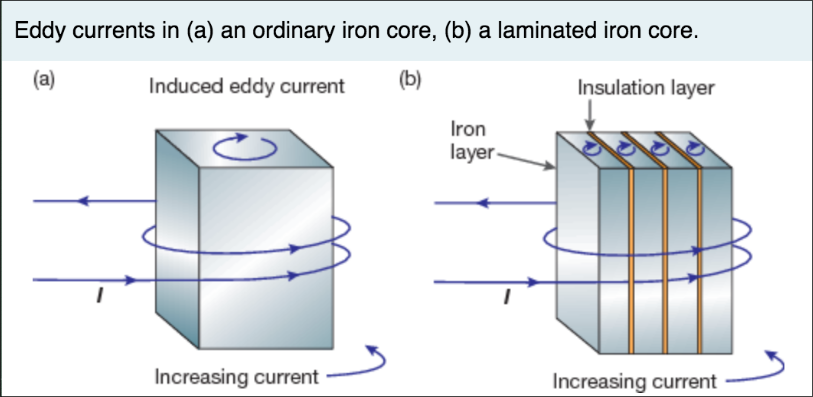
\includegraphics[width=15cm]{eddy_currents_in_transformer.png}
		\end{figure}

\section{Applications of Transformers} \label{20/03/2025}

	Power Distribution

	Resistance is due to:
	\begin{itemize}
		\item Length
		\item Material
		\item Temperature
		\item Thickness
	\end{itemize}

	\begin{align*}
		P_{in} &= IV \\
		P_{in} &= P_{out} + P_{loss} \\
		P_{loss} &= I^2 R = \frac{V^2}{R}
	\end{align*}

	Since the resistance due to material and distance is constant, $P_{loss}$ can be minimised by decreasing I and increasing V output which is done by a step-up transformer

	To minimise line loss: 
	\begin{itemize}
		\item Reduce resistance by using thicker wires
		\item Reduce current (high current $\rightarrow$ higher chance of collision) by stepping up voltage at the power plant
	\end{itemize}

	However, step-up transformers are only useful in distributing electricity over long distances. Step-down transformers must be used near the point of use to decrease the voltage.

\section{Generators}

	A generator is a device that \textbf{transforms mechanical energy into electrical energy}

	It is a backwards motor.

